   	\section{Geschäftsmodell}
   	Zur Beschreibung der Funktionsweise des zukünftigen Unternehmens und Evaluierung der optimalen Gewinnerwirtschaftung wurden drei Business Model Canvas erstellt. Dabei wurden die im Kapitel Personas und Anwendungsszenarien beschriebenen Zielgruppen betrachtet.

   	\begin{landscape}
	\newpage
	\subsection{Business Model Canvas - Persona-Typ: Wissenschaftler}
   	\begin{table}[h!]
		\begin{center}
			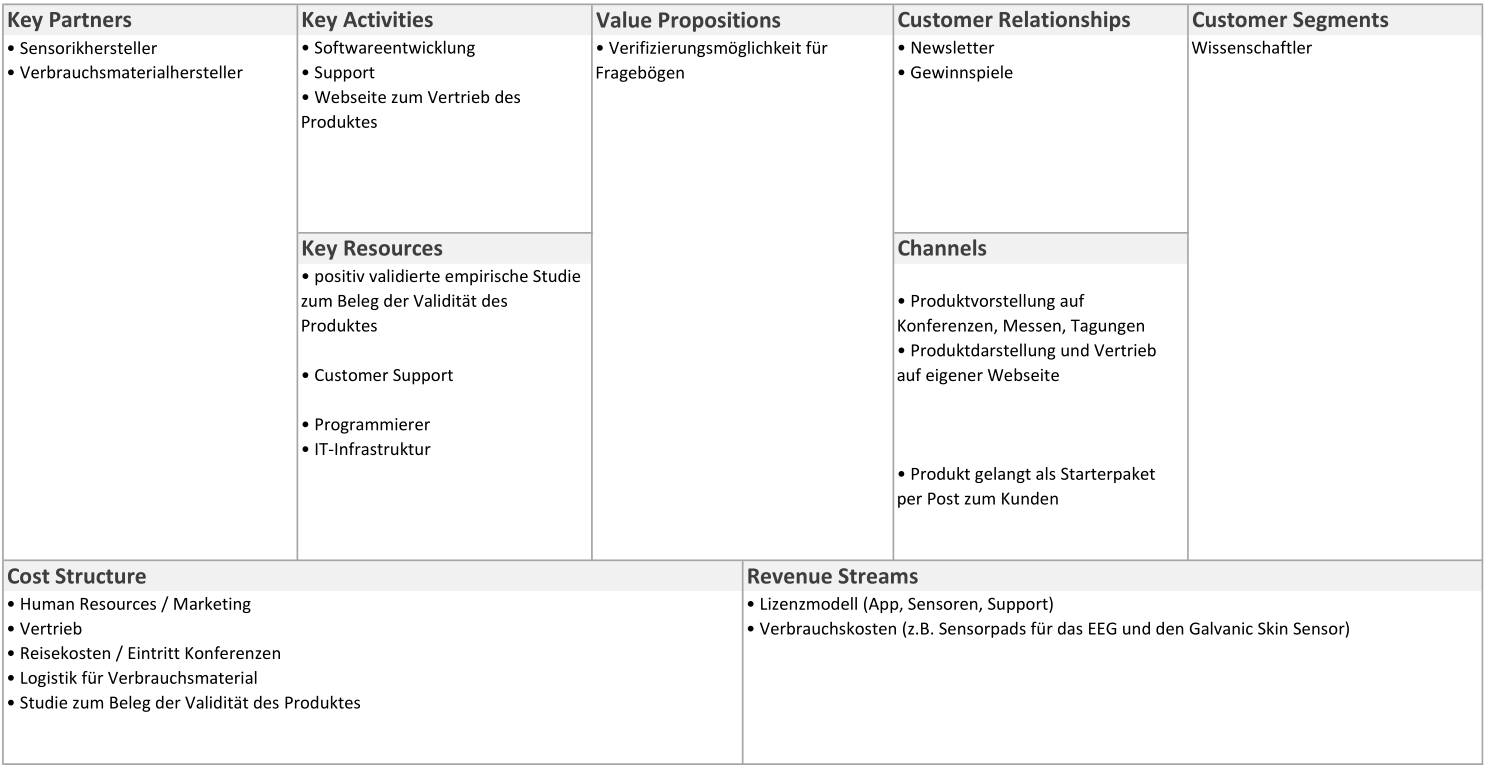
\includegraphics[width=1.3\textwidth]{business_canvas_1_wissenschftler.png}
		\end{center}
		\caption[Business Model Canvas - Persona-Typ: Wissenschaftler]{Business Model Canvas für die Persona vom Typ Wissenschaftler}
		\label{fig:business_model_1}
	\end{table}
	
	\newpage
   	\subsection{Business Model Canvas - Persona-Typ: Angeber}
   	\begin{table}[h!]
		\begin{center}
			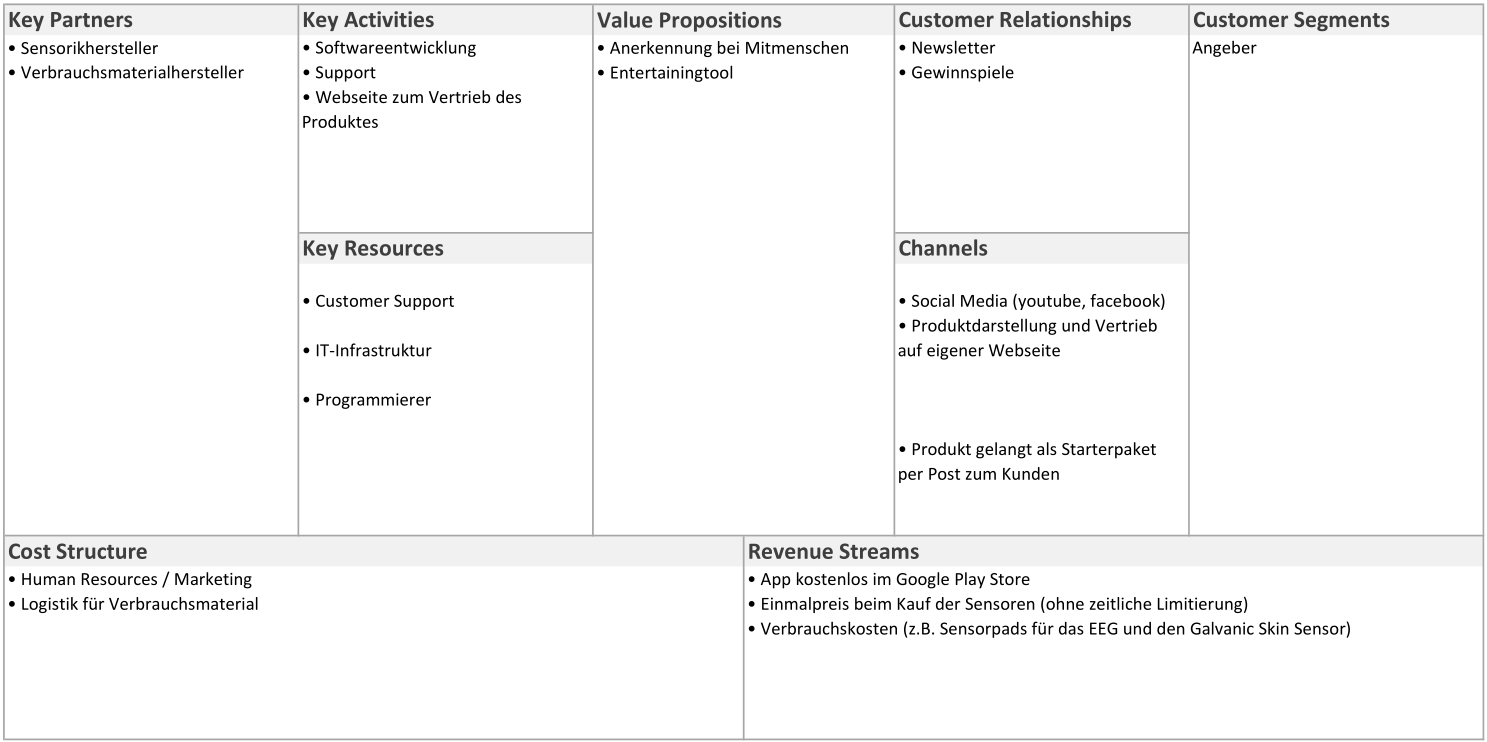
\includegraphics[width=1.3\textwidth]{business_canvas_2_angeber.png}
		\end{center}
		\caption[Business Model Canvas - Persona-Typ: Angeber]{Business Model Canvas für die Persona vom Typ Angeber}
		\label{fig:business_model_2}
	\end{table}
	
	\newpage
	\subsection{Business Model Canvas - Persona-Typ: Kontrollfreak}
   	\begin{table}[h!]
		\begin{center}
			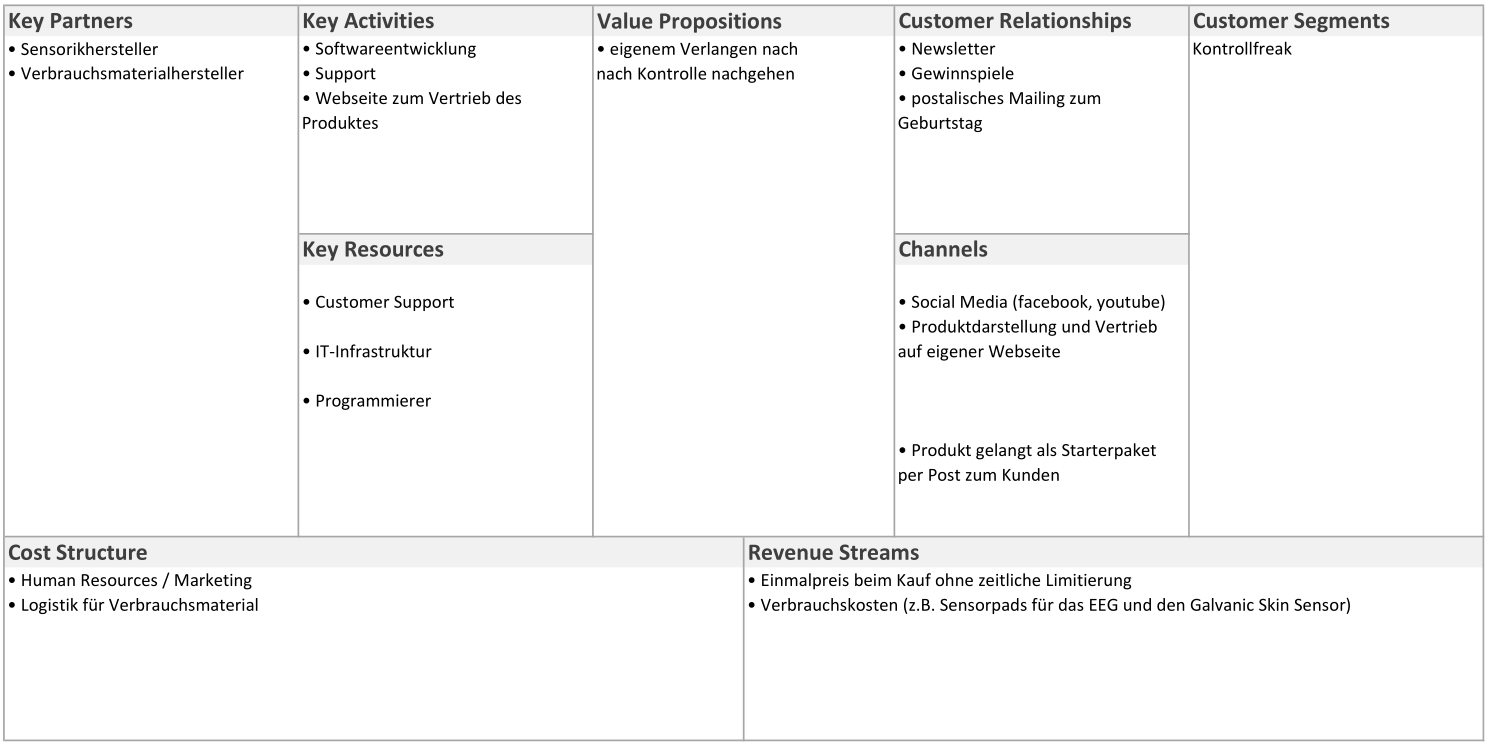
\includegraphics[width=1.3\textwidth]{business_canvas_3_kontrollfreak.png}
		\end{center}
		\caption[Business Model Canvas - Persona-Typ: Kontrollfreak]{Business Model Canvas für die Persona vom Typ Kontrollfreak}
		\label{fig:business_model_3}
	\end{table}

	\newpage
	\subsection{Fazit zum Geschäftsmodell}
	Als Fazit ergab sich, dass der Persona-Typ Wissenschaftler ein deutlich erhöhtes Ausmaß an Investitionen, wie beispielsweise Kosten für eine Studie zum Beleg der Validität des Produktes, benötigt. Da zudem Beschaffungsprozesse an der Universität einen langen Zeitraum andauern können, ergibt sich für das Unternehmen ein hoher finanzieller Aufwand und eine längere Zeit ohne Einnahmen. Dies ergibt ein hohes Risiko für unser Unternehmen und aus diesem Grund schließen wir dieses Geschäftsmodell aus. Der Persona-Typ Angeber kann nicht langfristig an unser Produkt gebunden werden und scheidet aus diesem Grund ebenfalls als Geschäftsmodell aus. Wir haben uns für eine Spezialisierung auf den Persona-Typ Kontrollfreak entschieden, da eine langfristige Bindung an unser Produkt und geringere Anfangskosten als beim Persona-Typ Wissenschaftler zu erwarten sind.

   	\begin{table}[h!]
		\begin{center}
			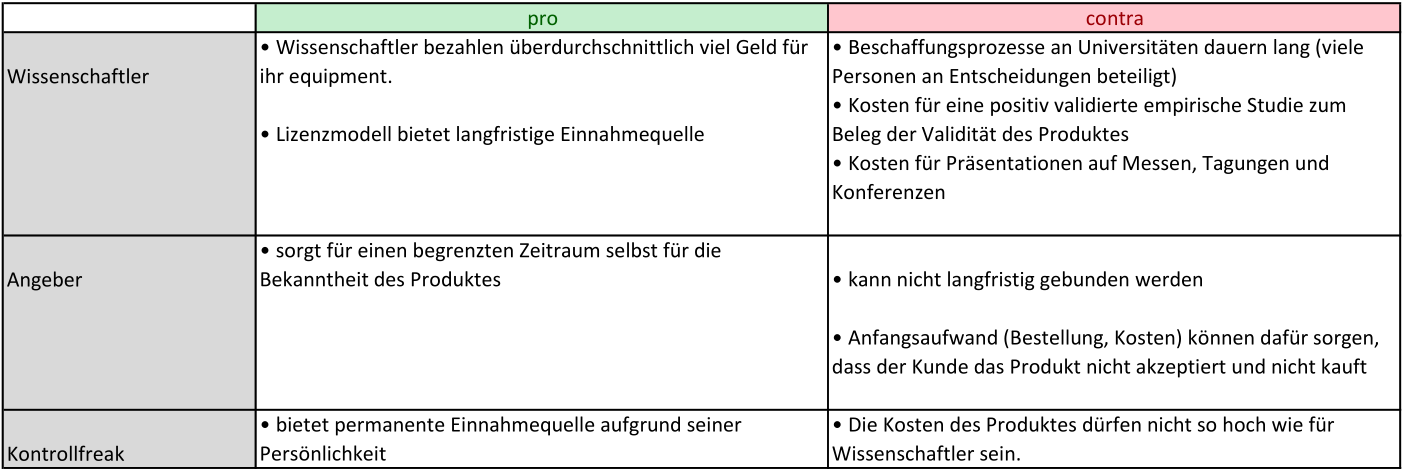
\includegraphics[width=1.1\textwidth]{business_canvas_4_pro_contra.png}
		\end{center}
		\caption[Business Model Canvas - Pro/Contra Auswertung]{Pro/Contra Auswertung der Business Model Canvas}
		\label{fig:business_model_2}
	\end{table}
	\end{landscape}
